\section{Difa Al Fansha}

\subsection{Teori}
	
	\subsubsection{Jelaskan apa itu klasifikasi teks, sertakan gambar ilustrasi buatan sendiri.}\hfill\\
Klasifikasi teks adalah proses mengelompokkan string ke beberapa kategori berdasarkan konten string.

	\begin{figure}[H]
		\begin{center}
		 
\includegraphics[width=10cm]{figures/1174076/figures4/1.png}
		 \caption{error}	
		\end{center}
	\end{figure}

	\subsubsection{Jelaskan mengapa klasifikasi bunga tidak bisa menggunakan machine learning, sertakan ilustrasi sendiri.}\hfill\\
Karena terdapat data noise, yang artinya tidak semua bunga memiliki ciri-ciri yang sama. Banyak bunga yang memiliki ciri serupa tetapi memiliki kategori yang berbeda.
Contoh : Komik one piece memiliki ciri-ciri genre Action, Adventure, dll. Tetapi tidak hanya one piece yang memiliki genre tsb, banyak komik yang memiliki genre serupa.
	\begin{figure}[H]
		\begin{center}
		 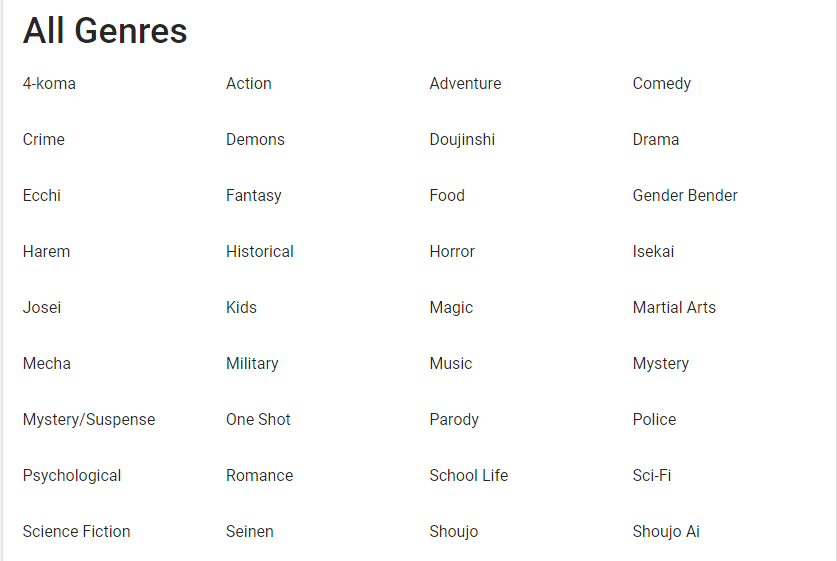
\includegraphics[width=10cm]{figures/1174076/figures4/2.png}
		 \caption{error}	
		\end{center}
	\end{figure}

	\subsubsection{Jelaskan bagaimana teknik pembelajaran mesin pada teks pada kata-kata yang digunakan di youtube,jelaskan arti per atribut data csv dan sertakan ilustrasi buatan sendiri.}\hfill\\
Menggunakan teknik bag-of-words pada klasifikasi berbasis text dan kata untuk mengklasifikasikan komentar yang ada di internet sebagai spam atau bukan. Misalkan pada kolom komentar dapat di cek seberapa sering suatu kata muncul dalam kalimat. Setiap kata dapat dijadikan baris dan kolomnya ini merupakan kategori kata tersebut, apakah masuk kedalam spam atau tidak. dan contoh lainnya yaitu pada Caption. dimana akan muncul subtitle secara otomatis dari youtube menggunakan sensor suara yang di sesuaikan dengan kata yang telah ditentukan.

	\begin{figure}[H]
		\begin{center}
		 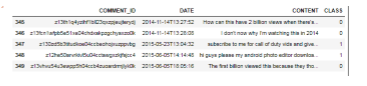
\includegraphics[width=10cm]{figures/1174076/figures4/3.png}
		 \caption{error}	
		\end{center}
	\end{figure}
	
	\subsubsection{Jelaskan apa yang dimaksud vektorisasi data.}\hfill\\
Vektorisasi merupakan proses konversi data. Vektorirasi membantu mengubah teks biasa kedalam bentuk vektor yang dapat dimengerti oleh komputer atau machine learning. Algoritma machine learning tidak bisa secara langsung menggunakan teks melainkan teks tersebut harus diubah menjadi angka. Kita membutuhkan cara untuk merepresentasikan data teks untuk algoritma pembelajaran mesin.
	
	\subsubsection{Jelaskan apa itu bag of words dengan kata-kata yang sederhana dan ilustrasi sendiri.} \hfill\\
Sebuah tas yang menampung kata-kata yang muncul dalam dokumen, lalu mengelompokkan data tsb kedalam perhitungan, berapakali sebuah kata muncul dalam satu kalimat.
	
	\begin{figure}[H]
		\begin{center}
		 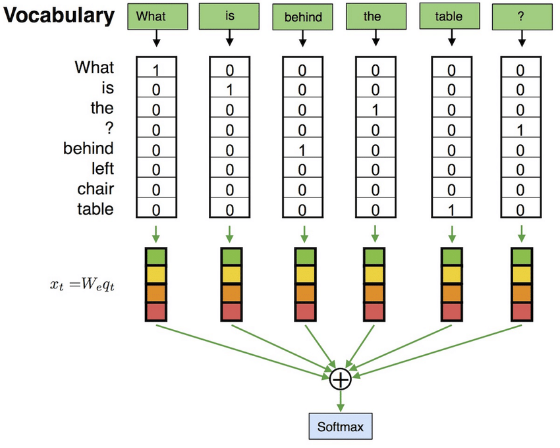
\includegraphics[width=10cm]{figures/1174076/figures4/4.png}
		 \caption{error}	
		\end{center}
	\end{figure}

	
	\subsubsection{Jelaskan apa itu TF-IDF, ilustrasikan dengan gambar sendiri.}\hfill\\
TF-IDF merupakan metode untuk menghitung bobot setiap kata pada suatu kalimat yang paling sering digunakan. TF-IDF ini akan menghitung nilai Term Frequency dan Inverse Document Frequency pada setiap kata dalam setiap kalimat yang muncul dengan diimbangi dengan jumlah dokumen dalam korpus yang mengandung kata. Contoh ilustrasi sederhananya seperti gambar berikut : 

	\begin{figure}[H]
		\begin{center}
		 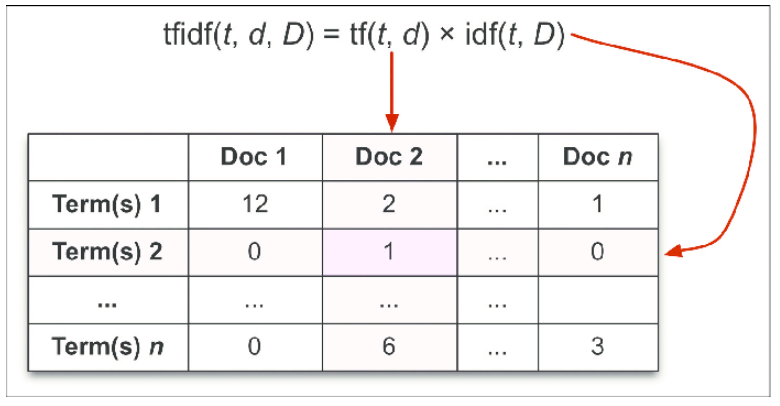
\includegraphics[width=10cm]{figures/1174076/figures4/5.png}
		 \caption{error}	
		\end{center}
	\end{figure}
	
\subsection{Praktek}

	\subsubsection{buat aplikasi sederhana menggunakan pandas, buat data dummy format csv sebanyak 500 baris dan melakukan load ke dataframe panda.jelaskan arti setiap baris kode yang dibuat(harus beda dengan teman sekelas)}\hfill\\
	
	\lstinputlisting[firstline=2, lastline=13]{src/1174076/src4/1174076.py}
	
	\begin{figure}[H]
		\begin{center}
		 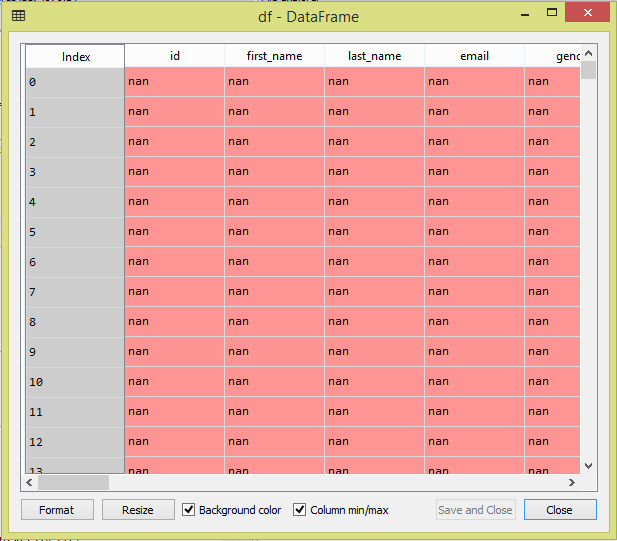
\includegraphics[width=10cm]{figures/1174076/figures4/6.png}
		 \caption{Soal nomor satu}	
		\end{center}
	\end{figure}	
	
	
	\subsubsection{ dari dataframe tersebut dipecah menjadi dua dataframe yaitu 450 row pertama dan 50 row sisanya(harus beda dengan teman sekelas)}\hfill\\

	\lstinputlisting[firstline=18, lastline=22]{src/1174076/src4/1174076.py}
	
	\begin{figure}[H]
		\begin{center}
		 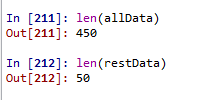
\includegraphics[width=10cm]{figures/1174076/figures4/7.png}
		 \caption{error}	
		\end{center}
	\end{figure}


	\subsubsection{pratekkan vektorisasi dan klasifikasi dari data (NPM mod 4, jika 0 maka katty perry, 1 LMFAO, 2 Eminem, 3 Shakira) dengan Decission Tree. Tunjukkan keluarannya dari komputer sendiri dan artikan maksud setiap luaran yang didapatkan.}\hfill\\
	
	\lstinputlisting[firstline=25, lastline=68]{src/1174076/src4/1174076.py}
	
	\begin{figure}[H]
		\begin{center}
		 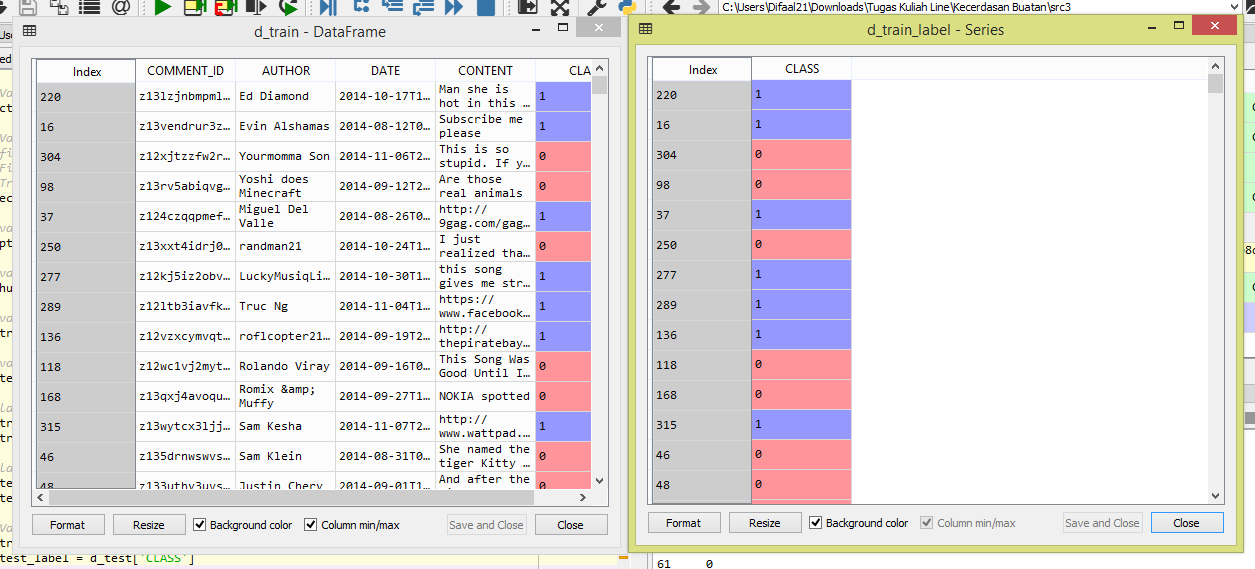
\includegraphics[width=10cm]{figures/1174076/figures4/8.png}
		 \caption{error}	
		\end{center}
	\end{figure}
	
	\subsubsection{Cobalah klasifikasikan dari data vektorisasi yang di tentukan di nomor sebelumnya dengan klasifikasi SVM. Tunjukkan keluarannya dari komputer sendiri dan artikan maksud setiap luaran yang didapatkan.}\hfill\\
	
	\lstinputlisting[firstline=72, lastline=82]{src/1174076/src4/1174076.py}
	
	\begin{figure}[H]
		\begin{center}
		 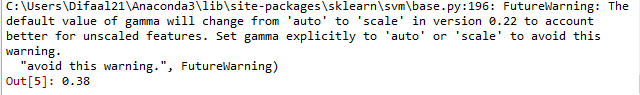
\includegraphics[width=10cm]{figures/1174076/figures4/9.png}
		 \caption{error}	
		\end{center}
	\end{figure}
		
	\subsubsection{Cobalah klasifikasikan dari data vektorisasi yang di tentukan di nomor sebelumnya dengan klasifikasi Decission Tree. Tunjukkan keluarannya dari komputer sendiri dan artikan maksud setiap luaran yang didapatkan.}\hfill\\
	
	\lstinputlisting[firstline=86, lastline=96]{src/1174076/src4/1174076.py}
		
	\begin{figure}[H]
		\begin{center}
		 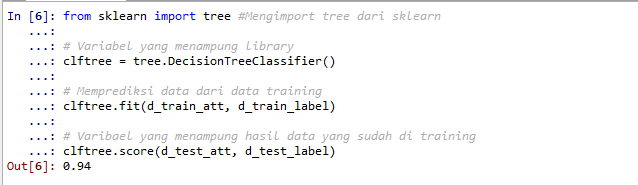
\includegraphics[width=10cm]{figures/1174076/figures4/10.png}
		 \caption{error}	
		\end{center}
	\end{figure}

	\subsubsection{Plotlah confusion matrix dari praktek modul ini menggunakan matplotlib.Tunjukkan keluarannya dari komputer sendiri dan artikan maksud setiap luaran yang didapatkan.}\hfill\\
	
	\lstinputlisting[firstline=101, lastline=142]{src/1174076/src4/1174076.py}
		
	\begin{figure}[H]
		\begin{center}
		 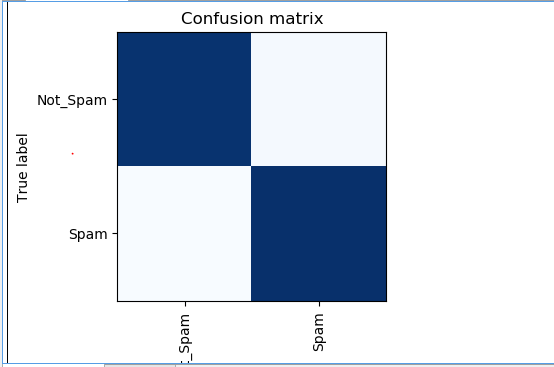
\includegraphics[width=10cm]{figures/1174076/figures4/11.png}
		 \caption{error}	
		\end{center}
	\end{figure}

	\subsubsection{jalankan program cross validaiton pada bagian teori bab ini. Tunjukkan keluarannya dari komputer sendiri dan artikan maksud setiap luaran yang didapatkan.}\hfill\\
	
	\lstinputlisting[firstline=145, lastline=160]{src/1174076/src4/1174076.py}
		
	\begin{figure}[H]
		\begin{center}
		 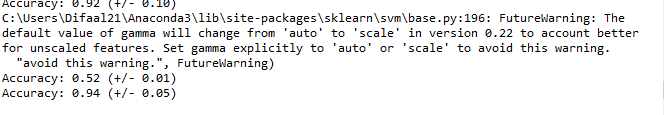
\includegraphics[width=10cm]{figures/1174076/figures4/12.png}
		 \caption{error}	
		\end{center}
	\end{figure}

	\subsubsection{Buatlah program pengamatan komponen informasi pada bagian teori bab ini. Tunjukkan keluarannya dari komputer sendiri dan artikan maksud setiap luaran yang didapatkan.}\hfill\\
	
	\lstinputlisting[firstline=165, lastline=178]{src/1174076/src4/1174076.py}
		
	\begin{figure}[H]
		\begin{center}
		 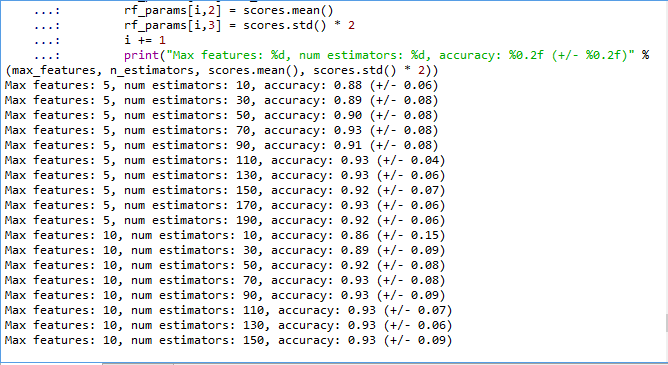
\includegraphics[width=10cm]{figures/1174076/figures4/13.png}
		 \caption{error}	
		\end{center}
	\end{figure}
	
\subsection{Penangan Error}
	
	\subsubsection{Screenshoots Error}\hfill\\
	
	\subsubsection{Tuliskan kode eror dan jenis errornya}\hfill\\
	 
	\subsubsection{Solusi pemecahan masalah error tersebut}\hfill\\
	
	
\subsection{Link Youtube}
	
	\subsubsection{}\hfill\\

	